\documentclass{amsart}

\usepackage{amsmath,amssymb}
\usepackage{amsthm}
\newtheorem*{theorem}{Theorem}

\usepackage{tikz}
\usetikzlibrary{shapes,snakes}
\usetikzlibrary{matrix}
\usetikzlibrary{calc}
\usetikzlibrary{positioning}

\title{Orthogonal Projections Notes}
\author{David E. James}

\begin{document}

\maketitle
Orthogonal Projections

\bigskip

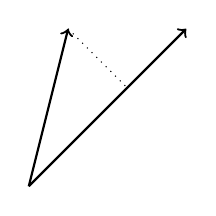
\begin{tikzpicture}
\coordinate (A) at (0,0);
\coordinate (B) at (2,2);
\coordinate (C) at (0.5,2);

\draw[->, thick] (A) -- (B);
\draw[->, thick] (A) -- (C);
\draw[dotted] (C) -- ($(A)!(C)!(B)$);
\end{tikzpicture}


\begin{theorem}[Orthogonal Decomposition Theorem]
Let some new statement about the theorem.
Let W be a subspace with orthogonal basis

\end{theorem}




\begin{theorem}[Best Approximation Theorem]

\end{theorem}


\begin{theorem}[Projection is a Linear Transform]

\end{theorem}


\end{document}
